\documentclass{article}

\usepackage[utf8]{inputenc}
\usepackage{mathtools}
\usepackage{amssymb}
\usepackage{amsmath}
\usepackage{amsthm}
\usepackage{enumitem}
\usepackage{tikz}
% \usetikzlibrary{patterns}

\usepackage{bbm}



\title{Discrete Geometrie I - Assignment 03}
\date{}
\author{Viet Duc Nguyen (395220)\\
    \underline{vd.nguyen96@gmail.com}
}



\begin{document}

\maketitle

\section*{Exercise 01}
Let $P_1$ and $P_2$ be two polyhedron in $\mathbb R^n$. Consider the operator $+: \mathbb R^{n \times n} \to \mathbb R^n, (x,y) \mapsto x+y$. That operator is linear.

\begin{enumerate}
    \item $P_1 \times P_2$ is a polyhedron. To see this, let $A_1 x \leq b_1$ and $A_2 x \leq b_2$ denote the linear inequalities that define $P_1$ and $P_2$. Then, 
    $$
        P_1 \times P_2 = \{ (x,y) \in \mathbb R^{n \times n} : A_1 x \leq b_1 \land A_2 y \leq b_2 \},
    $$
    which shows that $P_1 \times P_2$ is a polyhedron.
    \item $P_1 + P_2$ is the image of $P_1 \times P_2$ under the operator $+$. For applying a linear transformation on a polyhedra in $\mathbb R^n$ yields again a polyhedra, $P_1 + P_2$ is a polyhedra.
\end{enumerate}


\section*{Exercise 02}

First, we show that $T(P)$ solves the linear inequalities. Second, we show that the linear inequalities are contained in the image of $P$ under the linear transformation $T$.

\begin{enumerate}
    \item Let $Q = T(P)$ and $y \in Q$. Then there exists $x \in P$ such that $T(x) = y$, which implies 

    $$
        \langle c_i, y \rangle = \langle c_i, T(x) \rangle = \langle T^*(c_i), x \rangle = \langle a_i, x\rangle \leq b_i \quad \forall i = 1,...,m.
    $$

    \item Let $y \in \mathbb R^n$ such that $\langle c_i,y\rangle \leq b_i$ for all $i = 1,...,m$. Then, there is $x \in \mathbb R^n$ such that $T(x) = y$ since $T$ is bijective. We show that $x \in P$, and hence it follows that $y \in T(P)$. We claim $\langle a_i, x\rangle \leq b_i$ for all $i = 1,...,m$.

    $$
        \langle c_i, y \rangle = \langle c_i, T(x) \rangle = \langle T^*(c_i), x \rangle = \langle a_i, x\rangle \leq b_i \quad \forall i = 1,...,m.
    $$
\end{enumerate}




\section*{Exercise 03}
Let $A \subset \mathbb{R}^d$. 
\begin{enumerate}
    \item \textbf{Let $A$ be convex and open. Then, $A$ is algebraically open.} Let $L = \{ r + \tau s : \tau \in \mathbb{R}\}$ for any $r,s \in \mathbb{R}^d$. We want to show that 
    $$
        A \cap L = \{ r + \tau s : \tau \in I \},
    $$
    where $I$ must be an open interval.

    \begin{enumerate}
        \item $I$ is an interval, because $L$ and $A$ are convex and the intersection of convex sets yields a convex set. Hence, 
        $$
            A \cap L = \{ r + \tau s : \tau \in I \}
        $$
        must be convex. This set is convex if and only if $I$ is convex. Consequently, $I$ must be an intervall for the only convex sets in $\mathbb{R}^1$ are intervals.        

        \item Claim: $I$ is open. Let $x = r + \tau_0 s  \in A \cap L$ for some $\tau_0 \in \mathbb R$. To show that $I$ is open, we need to find an open neighborhood $\tau_0 \in U_\epsilon(\tau_0)$ with radius $\epsilon$ such that $r+\tau s \in A \cap L$ for all $\tau \in U_\epsilon(\tau_0)$.
        
        There exists an open neighborhood $U_{\delta}(x) \subset A$ with radius $\delta > 0$ since $A$ is open. Let $\epsilon = \frac{\delta}{||s||}$. Then, it holds for all $|\tau| < \epsilon$ that
        $$
            || x - \left(r + (\tau_0 + \tau) s\right)|| = ||\tau s|| < ||\frac{s}{||s||}\delta|| = \delta.
        $$
        This implies that 
        $$
            r + (\tau_0 + \tau) s \in U_\delta(x) \subset A \cap L.
        $$
        We found a neighborhood with the desired properties, and thus $I$ is open.
    \end{enumerate}

    We see that $I$ is an open interval. Hence, $A$ is algebraically open.

    \item \textbf{Let $A$ be algebraically open. Then, $A$ is convex and open.} By definition, $A$ is convex if $A$ is algebraically open. So, $A$ is convex. It remains to show that $A$ is open.
    
    Remember that $A$ is a subset in $\mathbb R^d$. Let $e_i$ denote the $i$-th unit vector for $i=1,...,d$. Let $x \in A$. We want to find an open neighborhood $U_\delta(x) \subset A$.

    Consider straight lines 
    $$
        L_i = \{ x  + \tau e_i : \tau \in \mathbb{R} \}, \quad i = 1,..., d,
    $$
    that when intersected with $A$ yields 
    $$
        A \cap L_i = \left\{ x + \tau e_i : \tau \in I_i \right\},
    $$
    where $I_i = (\alpha,\beta)$ is an open interval with $\alpha \in [-\infty, 0)$ and $\beta \in (0, \infty]$. Let $p_i^+ = x + \tau e_i$ with $\tau \in (\alpha,0)$ and $p_i^- = x + \tau e_i$ with $\tau \in (0, \beta)$. Then, consider the convex set 
    $$
        \mathrm{conv}\left(
            \bigcup_{i=1}^d \left\{ p_i^+, p_i^- \right\}
        \right).
    $$
    From the lecture we know that the interior of a convex set is convex. So, 
    \begin{align}\label{sponge}
        \mathrm{int}\left( \mathrm{conv}\left(
        \bigcup_{i=1}^d \left\{ p_i^+, p_i^- \right\}
    \right)\right)
    \end{align}
    is convex, too. That set is non-empty (the interior is non-empty, see exercise 5) and open. Furthermore, $A$ contains \eqref{sponge} since $A$ is convex. Thus, $\eqref{sponge}$ is an open neighborhood in $A$ containing $x$. We showed that $A$ is open.

    \begin{tikzpicture}[scale=1.5]
        \draw[dashed] (0,0.5)--(4,0.5) node[anchor=north east] {$A$}--(5,-1)--(2,-2.0)--(0,0.5);
        \draw[fill=black] (2,-1) circle (0.05) node[anchor=south west] {$x$};
        \draw (2,-1) -- (2, 1) node[anchor=west] {$L_1$};
        \draw (2,-1) -- (2, -3);
        \draw (2,-1) -- (0, -1);
        \draw (2,-1) -- (6, -1)node[anchor=south] {$L_2$};
        \draw[dashed] (2,-0.3) -- (3,-1) -- (2,-1.5) -- (1.5, -1)--(2,-0.3);
        \draw[fill=black] (2,-0.3) circle (0.05) node[anchor=south west] {$p_1^+$} (2,-1.5) circle (0.05) node[anchor=west] {$p_1^-$} (3,-1) circle (0.05) node[anchor=south] {$p_2^+$} (1.5,-1) circle (0.05) node[anchor=south] {$p_2^-$};
    \end{tikzpicture}
\end{enumerate}


\section*{Exercise 04}
Let $V = \left\{ (x_1,x_2,...) \subset \mathbb{R} : \text{$x_i \neq 0$ for finitely many $i$ } \right\}$. Let $A \subset V$ denote the sequence whose last non-zero entry is strictly positive.

\begin{enumerate}
    \item \textbf{$A$ is convex.} Let $(x_i)_{i \in \mathbb{N}}, (y_i)_{i \in \mathbb{N}} \in A$. Let $\alpha$ denote the last entry of $(x_i)$ that is non-zero; let $\beta$ denote the last entry of $(y_i)$ that is non-zero. We want to show that for all $\lambda \in [0,1]$ it holds
    $$
        (z_i) = \lambda(x_i) + (1-\lambda) (y_i) \in A.
    $$
    Without loss of generality, let $\alpha \geq \beta$. Then, $y_\alpha \geq 0$ because $(y_i) \in A$. Furthermore, $x_\alpha > 0$. Hence, $z_\alpha = \lambda x_\alpha + (1-\lambda) y_\alpha > 0$ for $\lambda \in [0,1]$. For $z_i$ with $i > \alpha$ it holds $z_i = \lambda x_i + (1- \lambda)y_i = 0$. To conclude, the last non-zero entry of $(z_i)$ is strictly positive, which implies $(z_i) \in A$.

    \item \textbf{There is no isolating hyperplane (we show a stronger statement).} Assume there is a linear functional $f: V \to \mathbb{R}$, $f \not \equiv \mathbf 0$ such that $f(\mathbf x) \geq \alpha$ for all $\mathbf x \in A$ for some fixed $\alpha \in \mathbb{R}$. Let $\mathbf z = (z_i) \in V$ be a sequence such that 
    \begin{itemize}
        \item $f(\mathbf z) \neq 0$
        \item $z_{i^*} > 0$, where $z_{i^*}$ is the last non-zero sequence member (if $z_{i^*} < 0$ just multiply the sequence with a negative scalar).
    \end{itemize}
    For $\mathbf z \in A$, it holds 
    $$
        f(\mathbf z) \geq \alpha.
    $$
    Now, consider the sequence $\mathbf{\tilde z}=(\tilde z_i) \in A$ defined as 
    \begin{align*}
        \tilde z_i &= \begin{cases}
            z_i \quad & i \leq i^* \\
            1 \quad & i = i^* + 1\\
            0 & \text{otherwise}
        \end{cases}\\  
        &\Downarrow \\
        (\tilde z_i) &= \left(z_1,z_2,...,z_{i^*},1,0,0,...\right).
    \end{align*}
    Again, it holds 
    $$
        f(\mathbf{\tilde z}) \geq \alpha.
    $$
    Here lies a contradiction. We decompose $\mathbf{\tilde z}$ into 
    $$
        \mathbf{\tilde z} = \mathbf z + \mathbf e_{i^*+1},
    $$
    where $\mathbf e_{i^*+1}$ denotes the ($i^*+1$)-th unit vector. Since $f$ is linear, it follows 
    \begin{align*}
        f(\mathbf{\tilde z}) = f(\mathbf{z}) + f(\mathbf{e_{i^* + 1}}) \geq \alpha.
    \end{align*}
    Here is the trick: we make use of the linearity of $f$ by multiplying the component $f(\mathbf{z})$ by a scalar such that the inequality $f(\mathbf{z}) + f(\mathbf{e_{i^* + 1}}) \geq \alpha$ does not hold anymore! Let $\iota \in \mathbb{R}$ denote that evil scalar, and define 
    $$
        \hat{\mathbf z} = \iota \mathbf{z} + \mathbf{e_{i^* + 1}}.
    $$
    By definition of $f$ it holds 
    $$
        f(\hat{\mathbf{z}}) \geq \alpha \quad \text{but} \quad f(\hat{\mathbf{z}}) \leq \alpha \text{ by construction of $\hat{\mathbf{z}}$}. 
    $$
    To conclude, whenever we find a sequence $\mathbf{z} \in V$ such that $f(\mathbf{z}) > 0$, we can multiply $\mathbf z$ with a scalar such that it is a member of $A$. Then, we can construct a contradiction. This implies that it holds $f(\mathbf z) = 0$ for all $\mathbf z \in V$. Thus, there cannot exist an isolating hyperplane, for hyperplanes are defined by linear functionals that are not identical to zero!

    \item \textbf{There is no hyperplane containing $A$.} This follows from 2., since if there is a hyperplane containing $A$ then we found an isolating hyperplane. But we showed that there is no isolating hyperplane!
\end{enumerate}


\section*{Exercise 05}
Let $\Delta \subset\mathbb R^n$ be a simplex. Let $a_1,...,a_{n+1}$ the affinely independent points that define the simplex. Without loss of generality, we can assume that one of the vertices is the origin, i.e. $a_{n+1} = 0 \in \mathbb R^n$. 

\begin{enumerate}
    \item We know from linear algebra that there exists a bijective linear transformation $T$ which transforms the simplex $\Delta$ to an unit cube $Q \subset \mathbb R^d$.
    \item The point $y = \sum^n_{i=1}\frac{1}{n}e_i$ lies in the unit cube.
    \item There is an open ball $U_1(y) \subset Q$ with radius $1$ which contains $y$.
    \item $T$ and $T^{-1}$ are continous because they are bounded (known from functional analysis). Hence, $T^{-1}(U_1(y))$ is an open subset of the interior of $\Delta$, which shows that $\mathrm{int}(\Delta)\neq \emptyset$.
\end{enumerate}

\iffalse
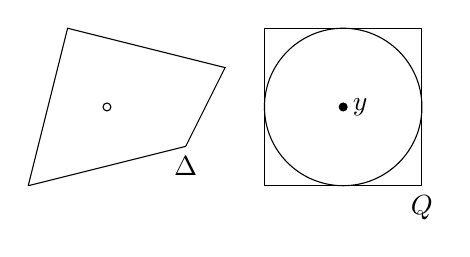
\begin{tikzpicture}
    \draw[shift={(-3,0)}] (0,0) -- (2, 0.5) -- (2.5,1.5) -- (0.5, 2) -- (0,0)  
    (2, 0.5) node[anchor=north] {$\Delta$} (1,1) circle (0.05) ;
    \draw (0,0) rectangle (2,2) (2,0) node[anchor=north] {$Q$};
    \draw (1,1) circle (1cm);
    \draw[fill=black] (1,1) circle (0.05)node[anchor=west] {$y$};
\end{tikzpicture}
\fi

\end{document}